\chapter{Literature Review}
\label{ch3_lit_review}
While there are multiple applications implemented in OpenCL, one such implementation that was studied as a part of related work is Portable Computing Language (POCL). It is portable and performance portable by virtue of a kernel compiler that can utilize the data parallelism of the program on different hardware architectures. Compiler transformations which produce work-group functions with multiple work items which can be parallelized are made by integrating the OpenCL implementation with LLVM compiler infrastructure. This newly implemented feature allows the kernels to be mapped to the parallel resources available on the different computing platforms
\cite{pocl}. The various experiments conducted by Pekka, J. et al on multiple hardware platforms showed that POCL could successfully port OpenCL applications efficiently.\newline\newline
Instruction Set Architecture (ISA) refers to the set of instructions which a processor understands to find the result of executing the instruction. It is an interface between a computer’s software and hardware which indicates the valid instructions that a machine can execute. Different architectures use different bit sizes, number of operands for specific instruction types and endianness, which affect their performance.\newline\newline
Complex Instruction Set Computers (CISC) architecture, a predecessor of RISC, aimed to complete a task in as few lines of assembly code as possible. This, however, requires processor hardware capable of understanding complex instructions. RISC emphasizes on software and uses only simple instructions that can be executed in a single clock cycle. RISC architecture also reduces the load on hardware space, allowing more general purpose registers to be used
\cite{risc_vs_cisc}. Intel x86 has retained CISC architecture due to other technological advancements, but is still considered too complex for simple projects.\newline \newline
RISC-V was developed with the need to meet the case for a free and open source ISA. For over 30 years, no other ISA has been a successful stack ISA including CISC. The existing CISC ISAs are being translated into easy to execute architectures while it was better to start off with an easy ISA. On this regard, RISC-V is better than its predecessors by removing unnecessary features like shift and keeping necessary load/store byte capabilities
\cite{riscv_isa_free}.\newline \newline
Several implementations of processors based on modified RISC-V architecture are present. Few of them are studied in this section. Berkeley Out of Order Machine (BOOM) is a synthesizable, superscalar and out-of-order RISC-V core written in Chisel, the hardware construction language
\cite{boom_2015}. Chisel stands for Constructing Hardware in a Scala Embedded Language. It supports a multi-core processor system by replacing the in-order Rocket core with the out-of-order BOOM core. It provides support for floating point, atomics and page-based virtual memory. It also supports supervisor mode and has a non-blocking data cache. It has a frequency greater than 2Hz.\newline \newline
PULPino is a Parallel Ultra Low Power Processor with a small single-core RISC-V System on Chip (SoC). It is a small part of PULP which is a huge energy efficient many-core SoC with multiple software framework support. PULPino focuses on simplicity by removing caches, memory hierarchy and DMA (Direct Memory Access). As seen from Figure \ref{fig:pulpino}, the processor has a single cycle access being directly connected to the instruction and data RAM. It consists an Advanced Peripheral Bus to allow easy addition of peripherals to the core. The Boot ROM loads the program from SPI Flash.

\begin{figure}[h!]
  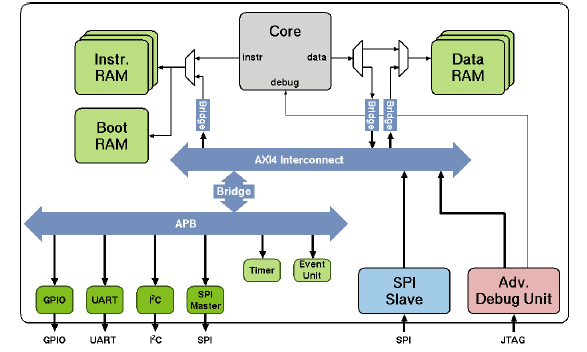
\includegraphics[width=\linewidth]{figures/pulpino.PNG}
  \caption{Architecture of PULPino single-core SoC
  \cite{pulpino}}
  \label{fig:pulpino}
\end{figure}

